\documentclass[10pt,professionalfont]{beamer}
\usepackage[utf8]{inputenc}
\usepackage[T1]{fontenc}
\usepackage[francais]{babel}
\usepackage{unicode}
\usepackage{booktabs}
\usepackage{lmodern,sfmath}
\DeclareUnicodeCharacter{2713}{\checkmark}

\makeatletter
\usetheme{CambridgeUS}%<<<
\definecolor{bleu}{rgb}{.1,.4,.6}%1a6699
\definecolor{rouge}{rgb}{.6,.1,.15}%991a26

\mode<presentation>{
\setbeamercolor{structure}{fg=rouge!80}
\setbeamercolor{palette primary}{fg=white,bg=rouge}
\setbeamercolor{palette secondary}{fg=white,bg=rouge!90}
\setbeamercolor{palette tertiary}{fg=white,bg=rouge!80}
\setbeamercolor{palette quaternary}{fg=white,bg=rouge!70}
\setbeamercolor{title}{fg=white,bg=bleu!60}
\setbeamercolor{section in head/foot}{fg=white,bg=bleu!90}
\setbeamercolor{subsection in head/foot}{fg=white,bg=bleu}
\setbeamercolor{frametitle}{fg=white,bg=bleu!80}
\setbeamercolor{titlelike}{parent=palette quaternary}
\setbeamercolor{block title}{fg=white,bg=bleu!80}
\setbeamercolor{block body}{fg=black,bg=bleu!20}
% couleurs perso pour ce qui suit
\setbeamercolor{strong}{fg=rouge}
\setbeamercolor{emph}{fg=bleu}
\setbeamercolor{table head}{fg=white,bg=bleu!80}
\setbeamercolor{table odd}{bg=bleu!20}
\setbeamercolor{table even}{bg=bleu!10}
}
\useinnertheme{rectangles}
\setbeamertemplate{blocks}[default]
\setbeamertemplate{title page}[default][rounded=false,shadow=false]
\setbeamertemplate{navigation symbols}{}


\defbeamertemplate{itemize item}{exemple}{{\color{bleu}$\rhd$}}
\defbeamertemplate{itemize subitem}{exemple}{{\color{bleu}$\rhd$}}
\newenvironment<>{exemple}{\begin{actionenv}%
  \ifnum\@itemdepth = 0 \setbeamertemplate{itemize item}[exemple]%
  \else \setbeamertemplate{itemize subitem}[exemple]\fi
  \begin{itemize}\item}%
  {\end{itemize}\end{actionenv}}
%>>>
\def\strong#1{{\usebeamercolor{strong}\textcolor{fg}{\textbf{#1}}}}
\def\imp#1{{\usebeamercolor{emph}\textcolor{fg}{\emph{#1}}}}
% Section frames%<<<
\let\oldsection\section
\newenvironment<>{sectionblock}[1]{%
  \begin{actionenv}#2\def\insertblocktitle{#1}%
  \mode<presentation>{%
    \setbeamercolor{block body}{fg=white,bg=rouge!90}
  }\usebeamertemplate{block begin}}%
{\par\usebeamertemplate{block end}\end{actionenv}}%
\newenvironment<>{subsectionblock}[1]{%
  \begin{actionenv}#2\def\insertblocktitle{#1}%
    \mode<presentation>{%
            \setbeamercolor{block body}{fg=white,bg=rouge!80}
    }\usebeamertemplate{block begin}}%
{\par\usebeamertemplate{block end}\end{actionenv}}%

\newif\if@sectionframe@cnt \@sectionframe@cnttrue
\def\sectionframe{\@ifstar
  {\@sectionframe@cntfalse\@sectionframe}%
  {\@sectionframe@cnttrue \@sectionframe}%
}
\def\thesection{\@Roman\c@section}
\def\thesubsection{\@arabic\c@subsection}
\def\@sectionframe#1{%
  \def\insertsectionhead{}\def\insertsubsectionhead{}\begin{frame}%
  \begin{center}\begin{sectionblock}{}\hfil\Large\strut
  \if@sectionframe@cnt \stepcounter{section}\thesection~--~\fi
  #1\end{sectionblock}
  \addtocounter{section}\m@ne
  \end{center}\end{frame}\section{#1}}
\def\subsectionframe#1{%
  \def\insertsubsectionhead{}\begin{frame}\begin{center}
  \begin{sectionblock}{}\hfil\Large\strut\insertsectionhead
  \end{sectionblock}
  \begin{subsectionblock}{}%
  \stepcounter{subsection}
  \hfil \large \thesubsection. #1\end{subsectionblock}
  \addtocounter{subsection}\m@ne
\end{center}\end{frame}\subsection{#1}}
%>>>
% Autoriser les blocs sans titre%<<<
\setbeamertemplate{block begin}{\par\medskip
 \ifx\insertblocktitle\empty\else
 \par\vskip\medskipamount%
  \begin{beamercolorbox}[colsep*=.75ex]{block title}
    \usebeamerfont*{block title}\insertblocktitle%
  \end{beamercolorbox}%
 {\parskip0pt\par}%
  \ifbeamercolorempty[bg]{block title}
  {}
  {\ifbeamercolorempty[bg]{block body}{}{\nointerlineskip\vskip-0.5pt}}%
 \fi
  \usebeamerfont{block body}%
  \begin{beamercolorbox}[colsep*=.75ex,vmode]{block body}%
    \ifbeamercolorempty[bg]{block body}{\vskip-.25ex}{\vskip-.75ex}\vbox{}%
}%>>>
\RequirePackage{colortbl}
% Playing with colortbl%<<<
% definining \tablecolor: the default color for a table
\let\orig@CT@setup\CT@setup
\let\CT@tablecolor\@empty
\let\CT@tablefg\@empty
\let\CT@rowfg\@empty
%
\def\tablecolor#1{\def\CT@tablecolor{#1}}
% defining \tablecoloralt: alternating colors for table rows
\let\CT@tablecoloraltI\@empty
\let\CT@tablecoloraltII\@empty
\def\tablecoloralt#1#2{\def\CT@tablecoloraltI{#1}\def\CT@tablecoloraltII{#2}}
\def\tablefg#1{\noalign{\gdef\CT@tablefg{#1}}}
\def\rowfg#1{\noalign{\gdef\CT@rowfg{#1}}}
% modifying start/save macros%<<<
\def\CT@start{%
  \let\CT@arc@save\CT@arc@
  \let\CT@drsc@save\CT@drsc@
  \let\CT@row@color@save\CT@row@color
  \let\CT@cell@color@save\CT@cell@color
  \let\CT@tablecoloraltI@save\CT@tablecoloraltI
  \let\CT@tablecoloraltII@save\CT@tablecoloraltII
  \def\CT@tablerowsave{\the\tablerow}\tablerow 0
  \def\+{\noalign{\CT@samerow}}%
  \global\let\CT@cell@color\relax}
\def\CT@end{%
  \global\let\CT@arc@\CT@arc@save
  \global\let\CT@drsc@\CT@drsc@save
  \global\let\CT@row@color\CT@row@color@save
  \global\let\CT@cell@color\CT@cell@color@save
  \let\CT@tablecoloraltI\CT@tablecoloraltI@save
  \let\CT@tablecoloraltII\CT@tablecoloraltII@save
  \expandafter \tablerow \CT@tablerowsave
}%>>>
\newcount\tablerow \def\CT@samerow{\global\advance\tablerow -1}
\CT@everycr{\noalign{\global\let\CT@row@color\relax
  \global\let\CT@rowfg\@empty
  \global\advance\tablerow 1}\the\everycr}
\def\CT@setup{\orig@CT@setup
  \ifx\CT@tablecoloraltI\@empty
    \ifx\CT@tablecolor\@empty\else\CT@color{\CT@tablecolor}\fi
  \else \ifodd\tablerow \CT@color{\CT@tablecoloraltI}%
    \else \CT@color{\CT@tablecoloraltII}\fi\fi
  \ifx\CT@rowfg\@empty \else
    \global\setbox\z@ \hbox{{\color{\CT@rowfg}\unhbox \z@}}\fi
  \ifx\CT@tablefg\@empty \else
    \global\setbox\z@ \hbox{{\color{\CT@tablefg}\unhbox \z@}}\fi
} % >>>
% Tableaux (utilise colortbl)%<<<
\newenvironment<>{tableau}[1]{\begin{actionenv}%
  \usebeamercolor{table head}
  \usebeamercolor{table odd}\usebeamercolor{table even}
  \def\entete{\+\rowcolor{table head.bg}\rowfg{table head.fg}}%
  \def\arraystretch{1.2}
  \tablecoloralt{table odd.bg}{table even.bg}\begin{tabular}{#1}}
  {\end{tabular}\end{actionenv}}
%>>>
% Macros perso
\def\abs#1{\left|#1\right|}
\def\pa#1{\left(#1\right)}
\def\acco#1{\left\{#1\right\}}
\def\bib#1{{\usebeamercolor{emph}\textcolor{fg}{~[#1]}}}
\def\F{\mathbb{F}}
\def\prob{\mathcal{P}}

\makeatother

\begin{document}
\title[Choix des courbes elliptiques]{Diversité et transparence : choix des courbes elliptiques}
\author[J.-P. Flori, J. Plût]{Jean-Pierre Flori, Jérôme Plût, Jean-René
Reinhard, Martin Ekerå}
\institute[ANSSI]{ANSSI/SDE/ST/LCR}

\begin{frame}<handout:0> \titlepage
\end{frame}
\sectionframe{Introduction}
\begin{frame}\frametitle{Les courbes elliptiques en cryptographie}
\begin{itemize}
\item Proposées en 1985 par Koblitz et Miller.
\item Fournissent un groupe abélien fini
où le logarithme discret est \strong{difficile}
(plus que dans les groupes multiplicatifs).
\item Standardisées à partir de 2000:
\begin{center}\begin{tableau}{lll}
\entete Année & Courbes & Tailles \\
2000 & NIST & 192, 224, 256, 384, 521\\
2005 & Brainpool & 160, 192, 224, 256, 320, 384, 512\\
2010 & OSCCA & 256 \\
2011 & ANSSI & 256 \\
\end{tableau}\end{center}
\item Plus quelques propositions académiques.
\item En pratique, on trouve surtout dans la nature les courbes NIST.
\end{itemize}
\end{frame}
\begin{frame}\frametitle{Pourquoi les courbes elliptiques ?}
\begin{itemize}
\item Un outil classique en cryptographie est
l'échange de clés de Diffie-Hellman, qui repose sur la relation
\[ (g^a)^b = g^{ab} = (g^b)^a, \]
valable dans le groupe multiplicatif des entiers modulo $p$.
\item La sécurité repose sur le problème du \strong{logarithme discret}:
étant donnés $g$ et~$g^a$, il est difficile de calculer $a$.
\item Ce groupe multiplicatif est cependant vulnérable
à certaines attaques (« crible algébrique »).
\item Solution : augmenter la taille de $p$...
\item ... ou alors, remplacer le groupe multiplicatif
par un groupe résistant à ces attaques.
\end{itemize}
\end{frame}
\begin{frame}\frametitle{Le groupe des points d'une courbe elliptique}
\begin{itemize}
\item Une courbe elliptique est donnée par l'équation
\[ y^2 = x^3 + a x + b \pmod{p}, \]
où $p$ est un nombre premier ($≠ 2,3$) et $a, b$ sont deux paramètres.
\item Les points de la courbe forment un groupe abélien
(noté additivement).
\item Le cardinal $N$ de ce groupe est environ $p$; en fait,
\[ \abs{N-(p+1)} ≤ 2√p. \]
\end{itemize}
\begin{block}{}
En général, le groupe des points d'une courbe elliptique
se comporte comme un « groupe générique » :
le logarithme discret a une complexité exponentielle.
\end{block}
Il est donc possible d'atteindre une sécurité de 128 bits
avec une taille de clé de 256 bits.
\end{frame}
\begin{frame}\frametitle{Pourquoi standardiser ?}
\begin{block}{}
\strong{En général,} le groupe des points d'une courbe elliptique
se comporte comme un « groupe générique » :
le logarithme discret a une complexité \strong{exponentielle}.
\end{block}
\begin{itemize}
\item Plus précisément, la complexité du logarithme discret
est dominée par $√{q}$, où $q$ est
le \imp{plus grand diviseur premier} du nombre de points de la courbe.
\begin{itemize}
\item Solution : avoir un nombre de points (presque) premier.
\end{itemize}
\item Certaines courbes particulières sont plus vulnérables :
le problème du logarithme discret peut être transféré
dans un groupe plus facile.
\begin{itemize}
\item Solution : éviter ces cas particuliers.
\end{itemize}
\end{itemize}

\begin{block}{}
Ces solutions sont gourmandes en calculs,
il n'est donc pas réaliste d'envisager
fabriquer une nouvelle courbe à la volée pour chaque échange.
\end{block}
\end{frame}
\begin{frame}\frametitle{Deuxième phase de standardisation}
Les premières courbes standardisées ont été produites
au début des années 2000, c'est-à-dire
une fois la recherche dans le domaine suffisamment avancée :
\begin{itemize}
\item possibilité de produire des courbes cryptographiques
(Schoof, Elkies, Atkin) ;
\item identification des classes de courbes faibles.
\end{itemize}
\begin{block}{}
À notre connaissance, ces courbes sont toujours sûres.
\end{block}
Mais de nouvelles préoccupations sont apparues depuis :
\begin{itemize}
\item doutes sur le processus de génération
(possibilité de publier une courbe secrètement vulnérable ?) ;
\item émergence des attaques latérales
(\emph{« side-channel attacks »}) ;
\item progrès scientifiques dans des domaines proches
(logarithme discret multiplicatif...).
\end{itemize}
\begin{block}{Juin 2015}
Le NIST organise un atelier sur le thème de
la standardisation des courbes elliptiques.
\end{block}
\end{frame}
\sectionframe{Sécurité}
\begin{frame}\frametitle{Aspects de la sécurité d'une courbe}
Qu'est-ce que qu'une « bonne » courbe pour la cryptographie ?
\begin{itemize}
\item Le problème du logarithme discret est difficile.
\item Les implémentations de la courbes sont résistantes
(par exemple aux attaques par canaux auxiliaires).
\item La courbe ne présente aucun signe particulier suspect.
\item Il est possible de réaliser des implémentations optimisées.
\item La courbe possède des propriétés particulières intéressantes.
\end{itemize}
\begin{block}{Conditions incompatibles}
Certaines de ces conditions sont incompatibles entre elles,
ce qui peut justifier l'existence de plusieurs (familles de) courbes.
\end{block}
\end{frame}
\subsection{Difficulté intrinsèque du logarithme discret}
\begin{frame}\frametitle{Difficulté du logarithme discret}
\begin{block}{}
Si le logarithme discret est facile, alors
toute implémentation de la courbe sera faible.
\end{block}
\begin{itemize}
\item Il existe des attaques contre des groupes génériques d'ordre $N$,
de complexité $√N$.
\item Pour qu'une courbe soit correcte,
on exige donc qu'il n'existe pas de meilleure attaque.
\end{itemize}
\begin{center}
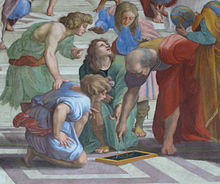
\includegraphics[width=.4\hsize]{raphael_euclid}
\end{center}
\end{frame}

\begin{frame}\frametitle{Notations}
Dans tout ce qui suit, $E$ désigne la courbe d'équation
\[ y^2 = x^3 + a x + b\]
définie sur le corps $k = \F_p$, et $N = \abs{E(\F_p)}$.
On considère la multiplication $n · P$ pour un scalaire $n$ secret.

On note $\prob(X)$ la probabilité d'un événement~$X$
comprise, selon le contexte,
sur l'ensemble des courbes sur $\F_p$ avec $p$ fixé,
ou sur l'ensemble des courbes sur $\F_p$ avec $p$ de taille fixée.
\end{frame}
\begin{frame}\frametitle{Courbes singulières}
Si $Δ = 4 a^3 + 27 b^2 = 0$, alors
la courbe d'équation $y^2 = x^3 + a x + b$ n'est pas une courbe elliptique :
c'est une cubique singulière.

Le groupe des points réguliers est alors isomorphe à
un groupe additif ou multiplicatif,
et le logarithme discret est sous-exponentiel, voire polynomial.

\begin{block}{}
Il est impératif que $Δ ≠ 0$ (ce qui arrive avec $\prob ≈ 1$).
\end{block}
\end{frame}
\begin{frame}\frametitle{Grand sous-groupe premier}
\begin{itemize}
\item Il existe des attaques génériques de complexité~$O(√q)$,
où $q$ est le plus grand diviseur premier de $N$.
\item Une courbe sûre doit donc avoir $q ≈ N$ ; idéalement, $q = N$.
\item Ceci nécessite de calculer $N$,
ce qui est une tâche relativement coûteuse.
\item La probabilité qu'une courbe aléatoire ait un ordre premier
est approximativement la même que celle
qu'un nombre aléatoire de la taille de $p$ soit premier,
soit $\prob ≈ \frac{1}{\log N}$.
\end{itemize}
\begin{block}{}
\begin{itemize}
\item Il est impératif que $N$ ait un grand facteur premier.
\item Calculer $N$ est l'une des étapes coûteuses
de la génération de la courbe.
\end{itemize}
\end{block}
\end{frame}
\begin{frame}\frametitle{Transfert additif ou multiplicatif}
\begin{itemize}
\item Si $N = p$ alors il existe un homomorphisme de groupe calculable
vers le groupe additif $\F_p$,
et donc le logarithme discret est de complexité polynomiale.
\begin{block}{}
Il est impératif que $N ≠ p$.
\end{block}
\item Cette condition exclut les courbes supersingulières.
\bigskip
\item Soit $e$ le \imp{degré de plongement},
c.-à-d. le plus petit entier tel que $N$ divise $p^e - 1$ ;
alors il existe un homomorphisme de groupe calculable vers
le groupe multiplicatif de $\F_{p^e}$,
et donc le logarithme discret a une complexité
sous-exponentielle relativement à $p^e$.

\begin{itemize}
\item Solution : si $e ≈ p$ alors cette
complexité est exponentielle relativement à $p$.
\end{itemize}
\end{itemize}
\begin{block}{}
\begin{itemize}
\item Il est impératif que $e$ soit assez grand ($\prob ≈ 1$).
\item
Pour calculer $e$, il faut connaître la factorisation de $q-1$,
ce qui est sous-exponentiel
(c'est asymptotiquement l'étape la plus coûteuse).
\end{itemize}
\end{block}
\end{frame}
\subsection{Résistance des implémentations de la courbe}
\begin{frame}
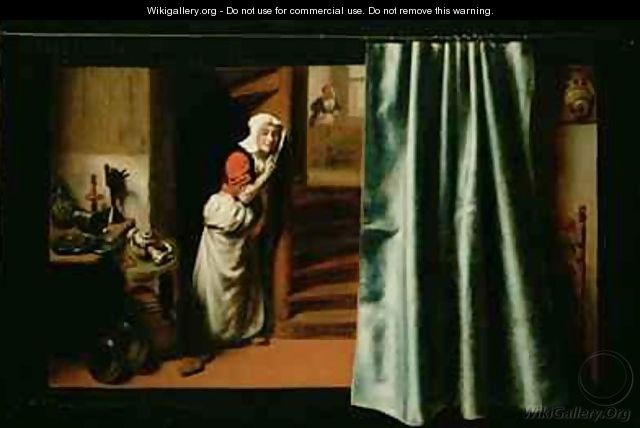
\includegraphics[width=.8\hsize]{maes_eavesdropping}
\end{frame}
\begin{frame}{Résistance des implémentations de la courbe}
\begin{block}{}
Il existe des courbes pour lesquelles,
bien que le logarithme discret soit difficile,
certaines implémentations ou certains protocoles sont faibles.
\end{block}
Exemple : multiplication par l'algorithme « doublement et addition »
non protégé.
\begin{center}
\includegraphics[width=24em,height=8em]{spa.pdf}
\hskip 1.2em
 \begin{tabular}{|p{1.45em}|p{1.45em}|p{1.45em}|p{1.45em}|p{1.45em}|p{1.45em}|p{1.45em}|p{1.45em}|} 
 \hline
 D&A&D&D& D&A&D&A\\
 \hline
 \multicolumn{2}{|c|}{1} &
 \vrule width 0pt height 2ex
 0 & 0 & \multicolumn{2}{|c|}{1} & \multicolumn{2}{|c|}{1} \\
 \hline
 \end{tabular}
\end{center}
\end{frame}
\begin{frame}\frametitle{Contre-mesures classiques}
\begin{itemize}
\item Contre les attaques simples :
élimination des branches conditionnelles sur un élément secret.
\begin{itemize}
\item double and always add :
\[ \begin{split}
&Q ← P;\\
&\texttt{for $i = ℓ-2,…,0$:}\\
&\qquad Q_0 ← 2 Q;\; Q_1 ← Q_0 + P;\; Q ← Q_{n_i};
\end{split} \]
\item échelle de Montgomery:
\[\begin{split}
&Q_0 ← P; Q_1 ← 2P;\\
&\texttt{for $i = ℓ-2,…,0$:}\\
&\qquad Q_{1-n_i} ← Q_0 + Q_1;\; Q_{n_i} ← 2 Q_{n_i};
\end{split}\]
\end{itemize}
\item Contre les attaques différentielles :
ne pas manipuler plusieurs fois le même élément secret.
\begin{itemize}
\item masquage aléatoire du secret ($n ← n + r · N$ avec $r$ aléatoire) ;
\item masquage aléatoire de la courbe ($a ← r^4 a, b ← r^6 b$) ;
\item masquage aléatoire du point ($(x:y:1) ← (rx:ry:r)$)...
\end{itemize}
\end{itemize}
\end{frame}
\begin{frame}\frametitle{Petit sous-groupe}
Si la courbe possède un petit sous-groupe, alors
il est possible, dans certains protocoles, d'obtenir de l'information
sur des données secrètes\bib{Lim-Lee 97}.
\begin{itemize}
\item Si le point de base $G$ est d'ordre $m$,
alors l'observation de $a G$ permet de retrouver la valeur $a \pmod{m}$.
\item Suppose un adversaire capable de fournir un point de base
de son choix.
\end{itemize}
\begin{block}{}
Il est préférable que le groupe des points de la courbe
soit d'ordre premier\\ ($\prob = 1$ si $N$ premier).
\end{block}
\end{frame}
\begin{frame}\frametitle{Sécurité de la courbe tordue}
La \imp{courbe tordue} de $E$ est la courbe~$E'$ d'équation
\[ d y^2 = x^3 + a x + b, \qquad
  \text{où $d$ n'est pas un carré dans~$\F_p$.} \]
Pour tout~$x ∈ \F_p$ tel que~$x^3+ax+b ≠ 0$,
il existe un point d'abscisse~$x$ sur
exactement une des deux courbes $E$ et~$E'$.

Dans certains cas, un adversaire peut injecter une abscisse appartenant
à la courbe tordue\bib{Fouque-Lercier-Réal-Valette 2008} :
\begin{itemize}
\item protocole mal conçu (compression de point),
\item manque de tests dans l'implémentation,
\item attaque par injection de faute...
\end{itemize}

\begin{block}{}
Il est préférable que la courbe tordue soit sûre.\\
($\prob ≈ \strong{$\frac{1}{\log p}$}$.)
\end{block}
\end{frame}
\begin{frame}\frametitle{Points spéciaux}
Un \imp{point spécial} est un point de la courbe
de la forme $(0, y)$ ou $(x, 0)$.

En présence de tels points, certaines implémentations
peuvent faire fuir de l'information\bib{Goubin 2003}.

\begin{itemize}
\item Des points spéciaux de la forme $(0, y)$ existent
si $b$ est un carré dans~$k$\\ ($\prob = 1/2$).
\item Des points spéciaux de la forme $(x, 0)$ existent
si $N$ est pair\\ ($\prob = 1$ si $N$ premier).
\end{itemize}


\begin{block}{}
Il est préférable que la courbe ne contienne pas de tels points spéciaux.
\end{block}
\begin{itemize}
\item Des points spéciaux de la forme $(0, y)$ existent toujours sur la courbe
ou sa tordue.\\ ($\prob = 1$).
\end{itemize}
\end{frame}
\begin{frame}\frametitle{Corps de base spéciaux}
De nombreuses courbes standard ont des corps de base spéciaux :
\[\begin{split} p_{192} &= 2^{192} - 2^{64} - 1\\
&= \texttt{\small 0xfffffffffffffffffffffffffffffffeffffffffffffffff}.
\end{split}\]
\begin{itemize}
\item Puisque $N = p + O(√p)$,
les premiers bits de~$N$ sont les premiers bits de~$p$.
\item Les premiers bits de $n + r · N$
sont les premiers bits de~$r$.
\item Ceci rend la protection par masquage de~$n$
insuffisante\bib{DK2005, BPSY2014, FRV2014, SW2015...}.
\end{itemize}

\begin{block}{}
Il est préférable que le corps de base ne soit pas d'une forme
spéciale.
\end{block}
\end{frame}
\begin{frame}\frametitle{Loi de groupe unifiée}
Certaines courbes admettent une loi d'addition \imp{unifiée} :
il existe un système de coordonnées permettant d'effectuer
les opérations $P + Q$, $2 P$, $P + 0$ par les mêmes formules.
\begin{itemize}
\item Courbes d'Edwards : $x^2 + y^2 = c^2 (t^2 + d z^2)$, $xy = zt$;
\item Courbes de Jacobi : $y^2 = z^2 + 2 a x^2 + b t^2$, $x^2 = zt$...
\end{itemize}

Ceci est possible sous certaines conditions sur la courbe :
\begin{itemize}
\item Edwards : point de $4$-torsion, $\prob = 17/48$;
\item Jacobi : point de $2$-torsion, $\prob = 2/3$...
\end{itemize}

Ceci ajoute une couche de protection contre les attaques simples.
\end{frame}
\subsection{« Généricité » de la courbe}
\begin{frame}\frametitle{Résistance à de possibles attaques futures}
\begin{itemize}
\item Et s'il existait des familles faibles ?
\item Éviter de produire des courbes trop « particulières ».
\item Vérifier des propriétés satisfaites avec~$\prob ≈ 1$.
\item En particulier, vérifier que différents nombres attachés à la
courbe sont « assez grands ».
\end{itemize}
\begin{center}
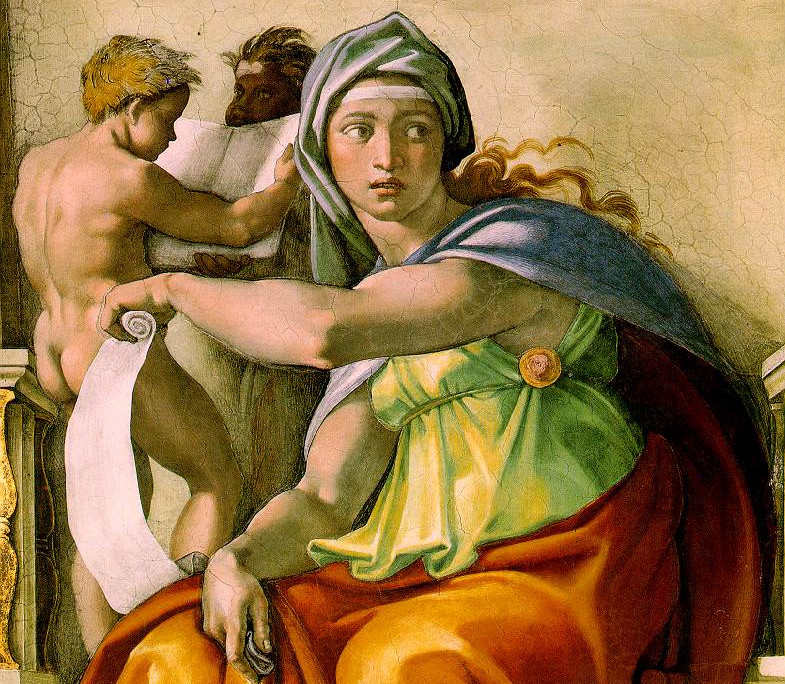
\includegraphics[width=.5\hsize]{michelangelo_sibyl}
\end{center}
\end{frame}
\begin{frame}\frametitle{Discriminant du corps des endomorphismes}
\begin{itemize}
\item Le \imp{corps des endomorphismes} de~$E$ est
l'extension quadratique~$K$ de~$ℚ$ engendrée par le Frobenius~$φ$.
\item Le polynôme minimal de~$φ$ est~$φ^2 - t φ + p$;
son discriminant est~$D_{φ} = t^2 - 4p < 0$.
\item Le discriminant de~$K$ est donné par $D_{φ} = D_{K} f_{φ}^2$,
où $D_{K}$ ou $D_{K}/4$ est sans facteur carré.
\end{itemize}
\begin{block}{}
En général, $\abs{D_K} ≈ p$ ;
en particulier, $\abs{D_{K}} ≥ √p$ avec~$\prob ≈ 1-O(1/√p)$.
\end{block}
\begin{itemize}
\item Cette condition élimine les valeurs~$D_{K} = -3$ et~$-4$,
correspondant aux $j$-invariants $0$ et~$1728$.
\end{itemize}
\end{frame}
\begin{frame}\frametitle{Nombre de classes}
Le nombre de classes~$h_K$ de~$K$ intervient dans divers
algorithmes liés à~$E$ :
\begin{itemize}
\item c'est le degré du polynôme de Hilbert à factoriser pour la
théorie de la multiplication complexe ;
\item c'est le plus petit degré d'une extension $L/ℚ$
sur laquelle $E$ admet un relèvement fidèle.
\end{itemize}
Ce nombre est minoré en fonction de $D_{K}$:
\[ h_K ≥ C \frac{\sqrt{\abs{D_K}}}{\log \abs{D_K}}. \]
\begin{itemize}
\item[$⇒$] aucune condition supplémentaire sur $h_K$ n'est a priori
nécessaire.
\end{itemize}
\end{frame}
\begin{frame}\frametitle{Friabilité du nombre de classes}
\begin{itemize}
\item Le nombre de classes $h_K$ est l'ordre du groupe de classes de~$K$.
\item Pour éviter de potentielles attaques utilisant la décomposition
de ce groupe en facteurs élémentaires, on souhaite que
$h_K$ ne soit pas friable (= n'ait pas que des petits facteurs premiers).
\item Un nombre aléatoire $n$ est $n^{1/u}$-friable avec
probabilité~$\prob ≈ u^{-u}$.
\item Par conséquent, $h_K$ a une probabilité négligeable d'être
$(\log p)^{O(1)}$-friable.
\begin{block}{}
En général, $h_K$ a au moins un diviseur premier~$≥ (\log p)^{O(1)}$.
\end{block}
\item Calculer (et factoriser) $h_K$ est sous-exponentiel\bib{Biasse
2010}, mais vérifier que $h_K$ n'est pas logarithmiquement friable
est polynomial.
\end{itemize}
\end{frame}
\begin{frame}\frametitle{Friabilité de la courbe tordue}
\begin{itemize}
\item Si la courbe $E$ a pour cardinal $N = p + 1 - t$,
alors sa tordue $E'$ a pour cardinal $N' = p + 1 + t$.
\item Le cardinal $N'$ est $p^{1/u}$-friable
avec probabilité $\prob ≈ u^{-u}$.
\begin{itemize}
\item Par exemple, $N'$ est $p^{1/4}$-friable avec probabilité $1/256$.
\end{itemize}
\begin{block}{}
En général, $N'$ a au moins un diviseur premier
de taille polynomiale en~$p$.
\end{block}
\item Le choix du seuil $u$ est délicat ; par exemple, pour $p≈
2^{256}$, une probabilité~$2^{-128}$ correspond aux nombres
$727$-friables...
\item Variante plus stricte de cette condition : $N'$ premier (= courbe
tordue sûre).
\end{itemize}
\end{frame}
\begin{frame}\frametitle{Corps de base spécial}
\begin{itemize}
\item Certaines courbes utilisent des corps de base
dont la cardinalité est un nombre premier « spécial » :
une valeur d'un « petit » polynôme.
\begin{exemple}
NIST $p_{192} = 2^{192} - 2^{64} - 1$ = $x^3 - x - 1$ où $x=2^{64}$.
\end{exemple}
\item Le logarithme discret \imp{multiplicatif} est plus facile
dans de tels corps que dans le cas général.
\item Il est envisageable que des attaques analogues soient découvertes
sur les courbes elliptiques.
\begin{block}{}
Il est souhaitable de choisir un nombre premier pseudo-aléatoire.
\end{block}
\item Il est impossible de  vérifier si un nombre
est une valeur d'un « petit » polynôme...
\end{itemize}
\end{frame}
\begin{frame}\frametitle{Degré de plongement}
\begin{itemize}
\item Le degré de plongement est l'ordre de $p$
dans le groupe multiplicatif $\F_q^{×}$.
\begin{block}{}
Le degré de plongement est~$≥ p^{1/4}$
avec probabilité~$\prob ≥ 1-1/√p$.
\end{block}
\end{itemize}
\end{frame}
\begin{frame}\frametitle{Structure multiplicative du corps de base}
\begin{itemize}
\item La structure multiplicative de $\F_p^{×}$ dépend
de la factorisation de~$p-1$.
\item Même si elle n'est pas liée au logarithme discret sur une courbe,
en général $p-1$ a au moins un grand diviseur premier.
\begin{block}{}
$p-1$ a un diviseur premier $≥ (\log p)^2$
avec probabilité $≥1-1/√p$.
\end{block}
\end{itemize}
\end{frame}
\begin{frame}\frametitle {Résumé}
\begin{center}\begin{tableau}{*{5}{l}}
\entete       & NIST & Brainpool & ANSSI & OSCCA\\
$N$ premier   &  ✓   & ✓         & ✓     & ✓   \\
$p$ ordinaire &      & ✓         & ✓     & ✓   \\
Loi unifiée   &      &           &       &      \\
$N'$ premier  &      &           &       &      \\
Générique & &✓&✓&✓ \\
\entete       & NUMS & Curve25519/41417 & Ed448-Goldilocks \\
$N$ premier   & & & & \\
$p$ ordinaire & & & & \\
Loi unifiée   &✓ &✓ &✓ & \\
$N'$ premier  &✓ &✓ &✓ & \\
Générique  & & & & \\
\end{tableau}\end{center}
\end{frame}
\subsection{Facilitation de l'implémentation}
\begin{frame}\frametitle{Facilitation de l'implémentation}
Certains choix de courbes permettent de disposer d'implémentations
plus rapides ou plus commodes.
\begin{center}
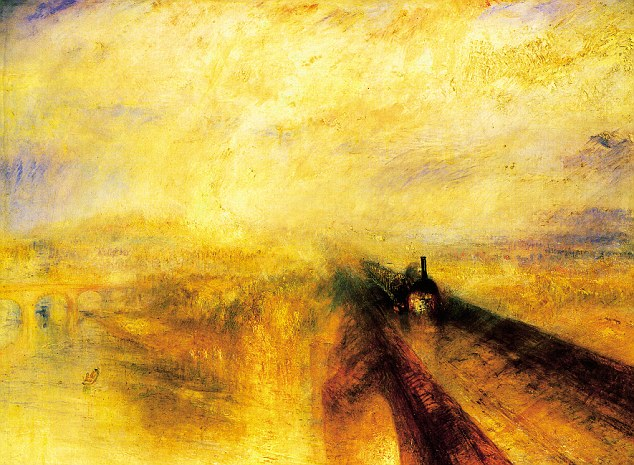
\includegraphics[width=.7\hsize]{turner_speed}
\end{center}
\end{frame}
\begin{frame}\frametitle{Coordonnées jacobiennes rapides}
Une courbe elliptique de la forme $y^2 = x^3 - 3 x + b$
(c'est-à-dire telle que $a=-3$)
permet d'économiser 2 des 10 multiplications requises
pour une addition de points.

\bigskip
Une courbe aléatoire sur $\mathbb F_p$ est isomorphe avec une courbe
$a=-3$ avec probabilité
\begin{itemize}
\item $\prob = 1/4$ si $p ≡ +1 \pmod{4}$,
\item $\prob = 1/2$ si $p ≡ -1 \pmod{4}$.
\end{itemize}
\end{frame}
\begin{frame}\frametitle{Nombre de points}
Si la courbe a $N < p$ points,
alors un élément de $ℤ/Nℤ$ peut être représenté par un nombre
de la même taille que $p$.

\bigskip
Exactement la moitié des courbes satisfont cette condition.
\end{frame}
\begin{frame}\frametitle{Racines carrées rapides}
Si $p ≡ -1 \pmod{4}$ (ou $p ≡ 5 \pmod{8}$) alors
calculer des racines carrées modulo~$p$ est plus facile,
ce qui permet de simplifier la compression de points.
\end{frame}
\begin{frame}\frametitle{Arithmétique dédiée}
\begin{itemize}
\item Certains choix de corps de base,
comme les nombres premiers « spéciaux » des courbes NIST,
permettent une arithmétique plus rapide.
\bigskip
\item De même, choisir des petites valeurs pour les paramètres $a$ et $b$
permet d'accélérer l'arithmétique de la courbe.
\end{itemize}
\end{frame}

\subsection{Diversité}
\begin{frame}\frametitle{Différents critères pour différents usages}
\begin{itemize}
\item Les critères précédemment énoncés ne peuvent être tous vérifiés.
\item En particulier, compromis vitesse/généricité.
\item Mais aussi, facilité d'implémentation/protection latérale.
\end{itemize}
\begin{block}{}
Il est souhaitable d'utiliser (et de normaliser) différentes courbes
pour différents usages !
\end{block}
\end{frame}

\begin{frame}\frametitle{Modèles usuels}
\begin{center}
\begin{tabular}{cc}
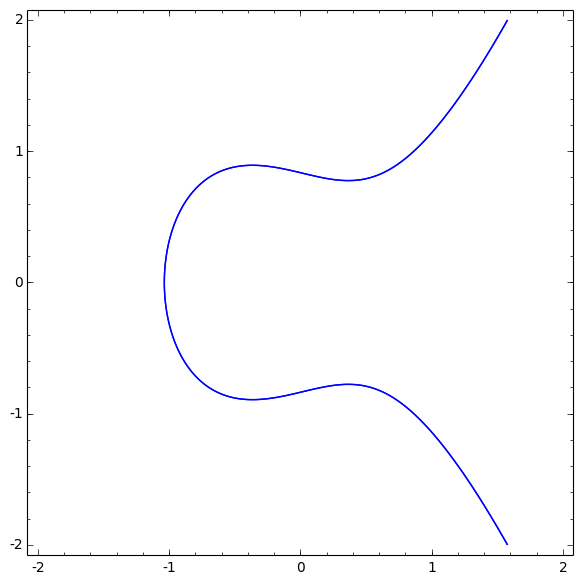
\includegraphics[width=.4\hsize]{weierstrass} & 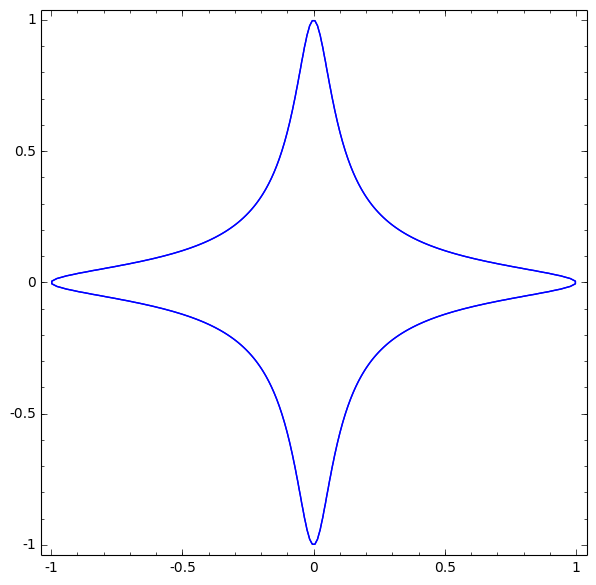
\includegraphics[width=.4\hsize]{edwards} \\
Weierstrass & Edwards \\
\end{tabular}
\end{center}
\end{frame}

\begin{frame}\frametitle{Modèles usuels}
\begin{center}
\begin{tabular}{cc}
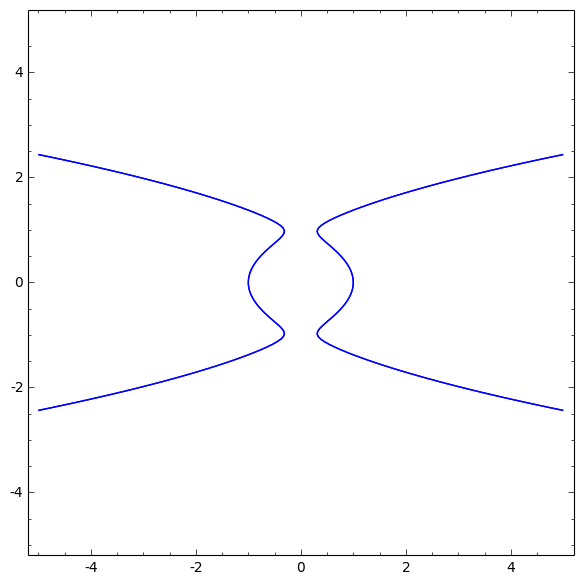
\includegraphics[width=.4\hsize]{jacobi} & 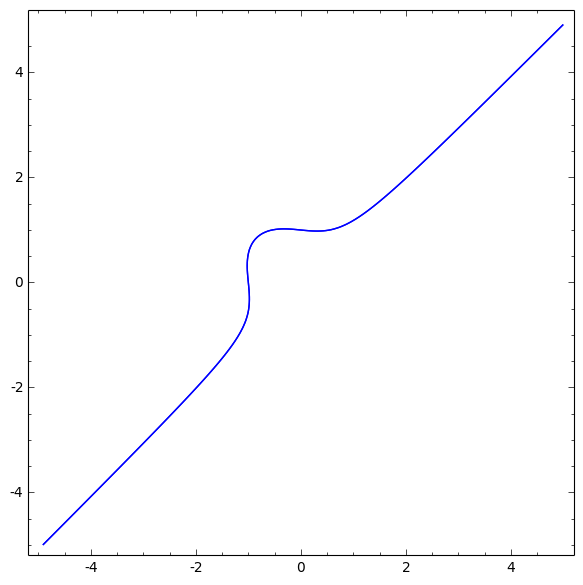
\includegraphics[width=.4\hsize]{hessian} \\
Jacobi & Hess \\
\end{tabular}
\end{center}
\end{frame}

\begin{frame}\frametitle{Sur un corps fini}
\begin{center}
\begin{tabular}{cc}
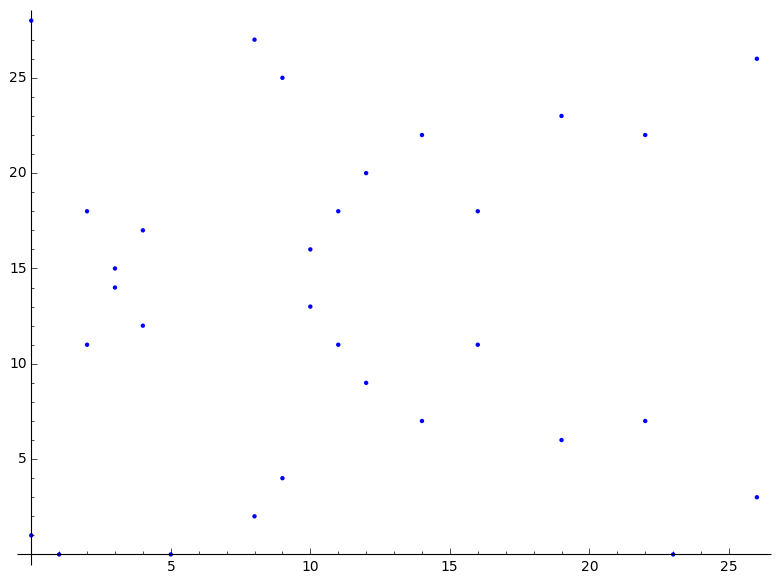
\includegraphics[width=.45\hsize]{frog} & 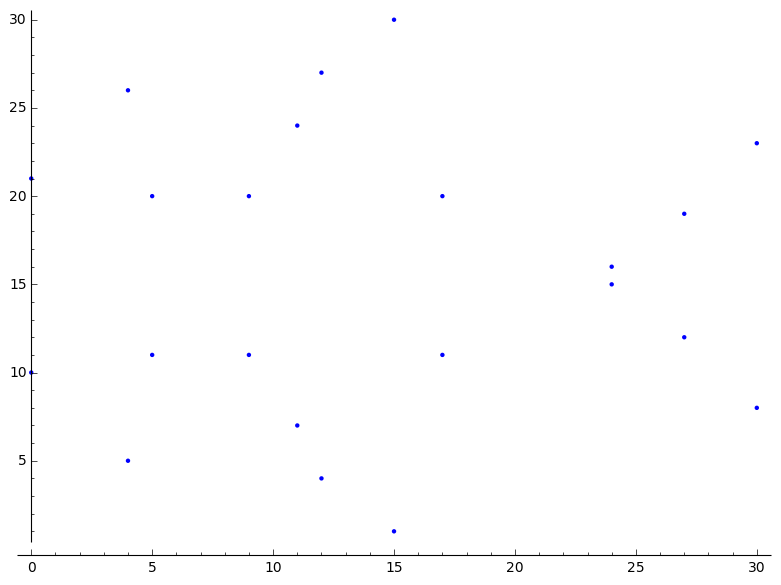
\includegraphics[width=.45\hsize]{cockroach} \\
Grenouille & Cafard \\
\end{tabular}
\end{center}
\end{frame}

\begin{frame}\frametitle{Sur un corps fini}
\begin{center}
\begin{tabular}{cc}
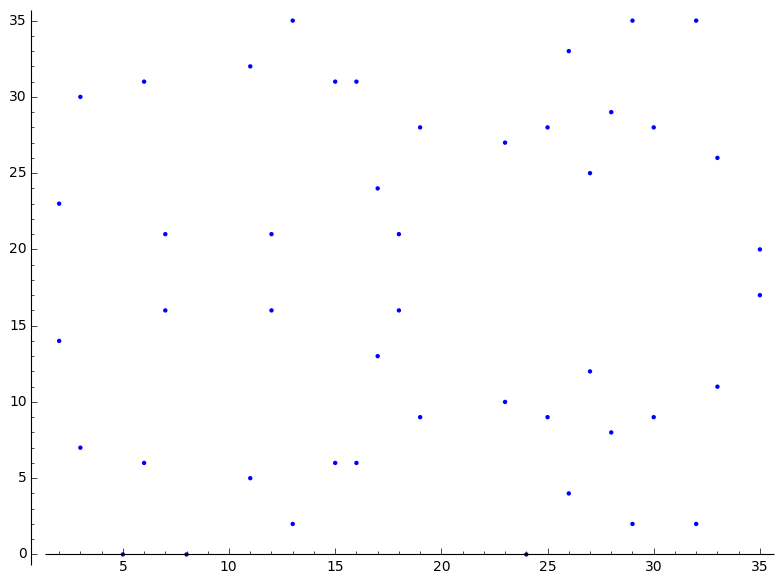
\includegraphics[width=.45\hsize]{walrus} & 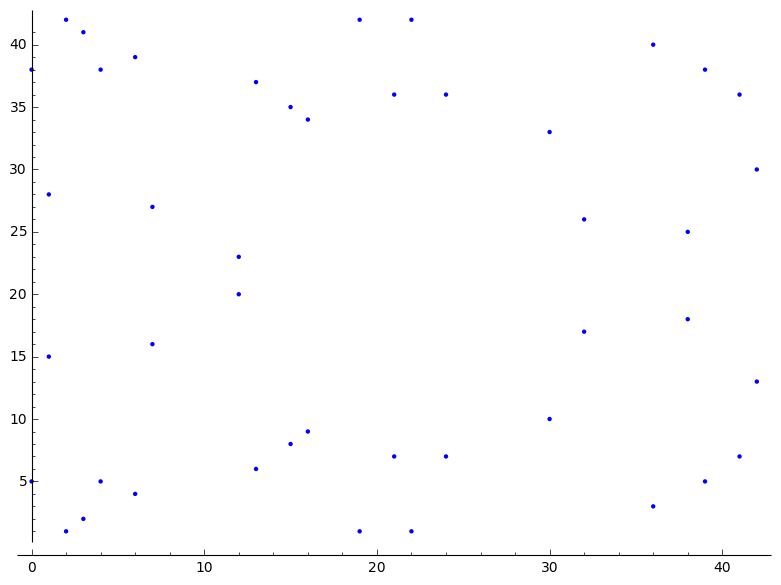
\includegraphics[width=.45\hsize]{bunny} \\
Morse & Lapin \\
\end{tabular}
\end{center}
\end{frame}

\sectionframe{Transparence}
\begin{frame}\frametitle{Transparence}
\begin{center}
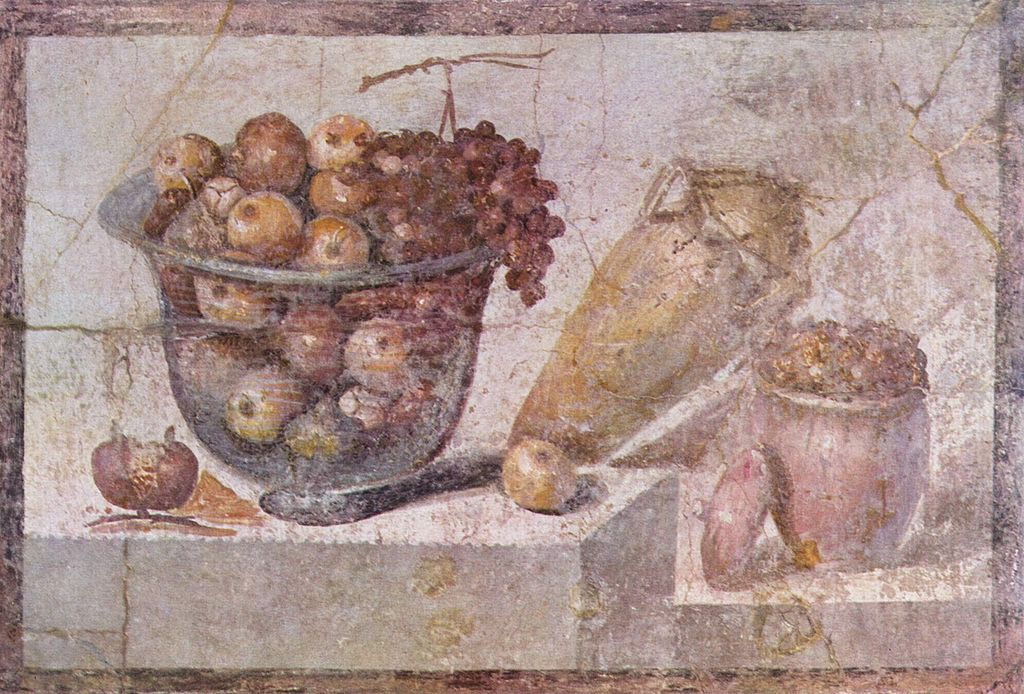
\includegraphics[width=.6\hsize]{pompeii_transparent}
\end{center}
\end{frame}
\subsection{Certificats de courbes elliptiques}
\begin{frame}\frametitle{Architecture}
\begin{itemize}
\item Fournir des courbes remplissant les conditions ci-dessus...
\item ... accompagnées d'un \strong{certificat} permettant
de vérifier les propriétés sans refaire tous les calculs :
\begin{itemize}
\item nombre de points,
\item discriminant et nombre de classes,
\item degré de plongement.
\end{itemize}
\bigskip
\item Programme \strong{déterministe} pour échantillonner une courbe.
\begin{itemize}
\item Processus de génération entièrement reproductible.
\item Peut être un générateur pseudo-aléatoire (généricité)
ou une énumération des petites valeurs (efficacité).
\item Certifier toutes les étapes du processus,
y compris les courbes rejetées.
\end{itemize}
\end{itemize}
\end{frame}
\begin{frame}\frametitle{Nombre de points premier}
\begin{itemize}
\item On connaît la borne de Hasse-Weil: $\abs{N-(p+1)} ≤ 2√p$.
\medskip
\item Si $G ≠ 0$ est tel que $q · G = 0$ avec $q ≥ p-2√p+1$ premier,
alors $q = N$.
\medskip
\item Certificat de primalité de $N$: $(G, q, Π)$,
où $Π$~est une preuve de primalité de~$q$.
\begin{itemize}
\item Pour les tailles usuelles de courbes elliptiques,
$Π$ peut être laissée vide ;
en effet, pour ces tailles, une preuve directe par APR-CL
est probablement plus rapide qu'une preuve par certificat ECPP.
\end{itemize}
\medskip
\item Ce certificat est produit une seule fois, pour la courbe finale.
\item Taille du certificat et vérification en $O(\log^2 p)$ opérations.
\end{itemize}
\end{frame}
\begin{frame}\frametitle{Nombre de points composé}
\begin{itemize}
\item Si $n < 2 (√p-1)^2$ est composé et si $P ≠ 0$, $n · P = 0$,
alors l'ordre de la courbe est composé.
\begin{itemize}
\item preuve: soit $d = \gcd (n, N)$; alors $d ≠ 1$ car~$P ≠ 0$.
Si $d ≠ N$ alors $d$~est un diviseur strict de~$N$.
Si $d = N$ alors $N$~divise~$n$ ; puisque $n/2 < (√p-1)^2$,
on a nécessairement~$N = n$, qui est composé.
\end{itemize}
\item Certificat de composition de~$N$ : $(n, c, P)$,
où $c$~est un témoin de composition (Miller-Rabin) de~$n$.
\item Complexité pour chacune des $O(\log p)$ ou $O(\log^2 p)$ courbes :
\begin{itemize}
\item production du certificat : $O(\log p)$~multiplications;
\item taille du certificat : $O(\log p)$;
\item vérification : $O(\log p)$~multiplications.
\end{itemize}
\end{itemize}
\end{frame}
\begin{frame}\frametitle{Nombre de points composé (II)}
\begin{itemize}
\item En pratique, le calcul du nombre de points $N$
se fait en calculant $N \pmod{ℓ}$ pour de petits nombres premiers~$ℓ$.
\item Si on trouve $N ≡ 0 \pmod{ℓ}$, on peut arrêter le calcul
pour cette courbe !
\bigskip
\item Dans ce cas, on trouve un polynôme $f_{ℓ}$, de degré~$O(ℓ)$,
dont les racines sont les abscisses de points de $ℓ$-torsion.
\item Trouver une racine de ce polynôme (par Cantor-Zassenhaus)
a un coût comparable à celui du calcul de $N \pmod{ℓ}$.
\item Dans ce cas, $(2ℓ, 2, P)$ est un certificat de composition.
\end{itemize}
\end{frame}
\begin{frame}\frametitle{Discriminant et nombre de classes}
\begin{itemize}
\item Le calcul du discriminant nécessite de factoriser
le nombre~$D_{φ} = t^2 - 4p$.
\item C'est asymptotiquement l'une des étapes dominantes
du processus de génération de la courbe ($L(1/3)$).
\item Certificat : la factorisation de $D_{φ}$.
\bigskip
\item Le calcul exact du nombre de classes est
probablement hors de portée ($L(1/2)$).
\item Il suffit d'un élément pour prouver que le nombre de classes est grand.
\item Il est impossible de prouver réalistement que la courbe
a été rejetée pour cause de nombre de classes trop petit.
\begin{exemple}
Solution : générer quelques éléments (déterministes) du groupe de classes
et prouver que l'on ne peut pas prouver avec ces éléments
que le nombre de classes est assez grand.
\end{exemple}
\end{itemize}
\end{frame}
\subsection{Le processus de génération}
\begin{frame}\frametitle{Exemple}
\begin{itemize}
\item Fonction d'échantillonnage pour une graine~$s$:
\begin{itemize}
\item $p$ = le plus petit premier $≥ s$;
\item $g$ = le plus petit générateur de $\F_p^{×}$;
\item courbes de la forme $y^2 = x^3 - 3x + b$, $b = 1, g, g^2, …$.
\end{itemize}
\item Conditions :
\begin{itemize}
\item $N$ et $N'$ premiers ;
\item $Δ ≠ 0$, $N ≠ p$;
\item degré de plongement de~$E$, $E'$ au moins~$p^{1/4}$;
\item nombre de classes $≥ p^{1/4}$.
\end{itemize}
\end{itemize}
\end{frame}
\begin{frame}\frametitle{Exemple de certificat}
Pour la graine $s = 2015$: $p = 2017$, $g = 2$,

\begin{block}{\small\tt Curve}\small\tt
(2017, -3, 625)\\
order = 2063, point = (0, 25)\\
twist\_order = 1973\\
disc\_factors = \{6043\}\\
class\_number = 9, form = (17,3,89)\\
embedding\_degree = 1031, factors = \{2, 1031\}\\
twist\_embedding\_degree = 493, factors = \{2, 17, 29\}
\end{block}
\vskip -1.7em

\begin{block}{\small\tt Rejected curves}\small\tt
((2017, -3, 5), composite, 2065, witness, 1679,
  point, (1,258))\\
((2017, -3, 25), torsion\_point, 3, point, (448, 288))\\
((2017, -3, 125), torsion\_point, 2, point, (982, 0))
\end{block}

\end{frame}
\begin{frame}\frametitle{Non-manipulabilité}
\begin{itemize}
\item Ce processus permet de produire \strong{déterministement}
une courbe elliptique cryptographique à partir
\begin{itemize}
\item d'un ensemble de conditions (y compris bornes numériques),
\item d'une fonction d'échantillonnage des courbes
(y compris graine éventuelle).
\end{itemize}
\item Seules quelques conditions influenceront probablement
le résultat final :
\begin{itemize}
\item sécurité de la courbe tordue,
\item choix des bornes de friabilité.
\end{itemize}
\item Pour éviter tout soupçon sur le choix de la graine :
\begin{itemize}
\item utiliser un schéma d'engagement sur des fragments de la graine ;
\item utiliser un résultat hors de portée de manipulation
(cours de la Bourse, résultat sportif, loterie publique).
\end{itemize}
\end{itemize}
\end{frame}

\begin{frame}\frametitle{Graine}
\begin{center}

\includegraphics[0.7\hsize]{keyboard_cat}
\end{center}
\end{frame}

\begin{frame}\frametitle{Questions ?}
\begin{center}
\includegraphics[width=.5\hsize]{roswell_speech}
\end{center}
\end{frame}
\end{document}
